\documentclass[a4paper]{article}
\usepackage[letterpaper, margin=1in]{geometry} % page format
\usepackage{listings} % this package is for including code
\usepackage{graphicx} % this package is for including figures
\usepackage{amsmath}  % this package is for math and matrices
\usepackage{amsfonts} % this package is for math fonts
\usepackage{tikz} % for drawings
\usepackage{hyperref} % for urls
\usepackage{stackengine}

\newcommand\tab[1][0.5cm]{\hspace*{#1}}

\title{Homework 2}
\author{Kaitlyn Mulligan}
\date{3/6/19}

\begin{document}
\lstset{language=Python}

\maketitle

\section{Instructions}
This assignment could be written in \LaTeX, just as the last homework assignment could 
have been.  Write in understandable, easy to follow English.  Make sure you provide good 
illustrations and figures.  Remember to include your Python programs in your assignment.\\
\tab Your assignment should be submitted in two ways: through GitHub, and in hardcopy (in 
class).  Use the \textbf{same} repository you have been using and submit your work in a 
folder named "\verb|lastname-xx|", where lastname is your last name \verb|xx| is the number 
of the assignment.

% ----------------------------------------------------------------------------------------------

\section{Problem Set}
The following is a list of problems you will solve.  These are from your textbook.  When 
providing your solutions (hopefully using \LaTeX), do not simply give the final answer, show 
how you arrived to the solution, justify your assumptions, and explain your results clearly.
\begin{itemize}
    \item \textbf{Problem 2.1}. \textit{Hint:} it suffices to make $\epsilon(M, N, \delta) = 
    \sqrt{\frac{1}{2N} \ln \frac{2M}{\delta}} \leq \epsilon$ and solve for $N$.
    \item \textbf{Problem 2.11}. \textit{Hint:} you should use Equation (2.12) and remember 
    that a confidence of $90\%$ means a $\delta = 0.1$.
    \item \textbf{Problem 2.12}. \textit{Hint:} use Equation (2.13).
    
    For the following two problems you may use the dataset generator downloadable on iLearn:\\
    \verb|Resources/Homework/2/makeSemiCircles.py|
    \item \textbf{Problem 3.1}
    \item (extra credit) \textbf{Problem 3.2}
\end{itemize}

% ----------------------------------------------------------------------------------------------

\subsection{Problem 2.1} In Equation (2.1), set $\delta = 0.03$ and let
\begin{equation*}
    \epsilon(M, N, \delta) = \sqrt{\frac{1}{2N} \ln \frac{2M}{\delta}}.
\end{equation*}
\begin{itemize}
    \item[(a)] For $M = 1$, how many examples do we need to make $\epsilon \leq 0.05$?\\
    We have that $\epsilon(M, N, \delta) = \sqrt{\frac{1}{2N} \ln \frac{2M}{\delta}} \leq 
    \epsilon$.  We also have that $M=1$ and $\delta = 0.03$.  We need to find $N$ when 
    $\epsilon \leq 0.05$.  Thus we have $\sqrt{\frac{1}{2N} \ln \frac{2M}{\delta}} \leq 
    \epsilon \leq 0.05$ or $\sqrt{\frac{1}{2N} \ln \frac{2M}{\delta}} \leq 0.05$.  Solving 
    for $N$ we have:
    \begin{align*}
        \sqrt{\frac{1}{2N} \ln \frac{2M}{\delta}} &\leq 0.05\\
        \sqrt{\frac{1}{2N} \ln \frac{2(1)}{0.03}} &\leq 0.05\\
        \frac{1}{2N} \ln \frac{2}{0.03} &\leq 0.0025\\
        \frac{1}{2}\ln \frac{2}{0.03} &\leq 0.0025N\\
        \frac{1}{2(0.0025)}\ln \frac{2}{0.03} &\leq N\\
        839.9410 &\leq N.
    \end{align*}
    Thus, $N = 840$.
    \item[(b)] For $M = 100$, how many examples do we need to make $\epsilon \leq 0.05$?\\
    We have that $\epsilon(M, N, \delta) = \sqrt{\frac{1}{2N} \ln \frac{2M}{\delta}} \leq 
    \epsilon$.  We also have that $M=100$ and $\delta = 0.03$.  We need to find $N$ when 
    $\epsilon \leq 0.05$.  Thus we have $\sqrt{\frac{1}{2N} \ln \frac{2M}{\delta}} \leq 
    \epsilon \leq 0.05$ or $\sqrt{\frac{1}{2N} \ln \frac{2M}{\delta}} \leq 0.05$.  Solving 
    for $N$ we have:
    \begin{align*}
        \sqrt{\frac{1}{2N} \ln \frac{2M}{\delta}} &\leq 0.05\\
        \sqrt{\frac{1}{2N} \ln \frac{2(100)}{0.03}} &\leq 0.05\\
        \frac{1}{2N} \ln \frac{200}{0.03} &\leq 0.0025\\
        \frac{1}{2} \ln \frac{200}{0.03} &\leq 0.0025N\\
        \frac{1}{2(0.0025)} \ln \frac{200}{0.03} &\leq N\\
        1760.9751 &\leq N.
    \end{align*}
    Thus, $N = 1761$. 
    \item[(c)] For $M = 10,000$, how many examples do we need to make $\epsilon \leq 0.05$?\\
    We have that $\epsilon(M, N, \delta) = \sqrt{\frac{1}{2N} \ln \frac{2M}{\delta}} \leq 
    \epsilon$.  We also have that $M=10,000$ and $\delta = 0.03$.  We need to find $N$ when 
    $\epsilon \leq 0.05$.  Thus we have $\sqrt{\frac{1}{2N} \ln \frac{2M}{\delta}} \leq 
    \epsilon \leq 0.05$ or $\sqrt{\frac{1}{2N} \ln \frac{2M}{\delta}} \leq 0.05$.  Solving 
    for $N$ we have:
    \begin{align*}
        \sqrt{\frac{1}{2N} \ln \frac{2M}{\delta}} &\leq 0.05\\
        \sqrt{\frac{1}{2N} \ln \frac{2(10000)}{0.03}} &\leq 0.05\\
        \frac{1}{2N} \ln \frac{20000}{0.03} &\leq 0.0025\\
        \frac{1}{2} \ln \frac{20000}{0.03} &\leq 0.0025N\\
        \frac{1}{2(0.0025)} \ln \frac{20000}{0.03} &\leq N\\
        2682.0091 &\leq N.
    \end{align*}
    Thus, $N = 2683$.  
\end{itemize}

% ----------------------------------------------------------------------------------------------

\subsection{Problem 2.11} Suppose $m_\mathcal{H}(N) = N + 1$, so $d_{VC} = 1$.  You have 
$100$ training examples.  Use the generalization bound to give a bound for $E_{\text{out}}$ 
with confidence $90\%$.  Repeat for $N = 10,000$.

Equation (2.12) states that $E_{\text{out}}(g) \leq E_{\text{in}}(g) + \sqrt{\frac{8}{N} \ln 
\frac{4m_{\mathcal{H}}(2N)}{\delta}}$.  Here we have $N = 100$, $m_{\mathcal{H}} = 100 + 1 = 101$, 
and $\delta = 0.1$.  Plugging these values in, we can use the generalization bound to give a bound 
for $E_{\text{out}}$ with confidence $90\%$.  We have:
\begin{align*}
    E_{\text{out}}(g) &\leq E_{\text{in}}(g) + \sqrt{\frac{8}{N} \ln \frac{4m_{\mathcal{H}}(2N)}
    {\delta}}\\
    E_{\text{out}}(g) &\leq E_{\text{in}}(g) + \sqrt{\frac{8}{100} \ln \frac{4(101)(2(100))}{0.1}}\\
    E_{\text{out}}(g) &\leq E_{\text{in}}(g) + \sqrt{\frac{8}{100} \ln \frac{80800}{0.1}}\\
    E_{\text{out}}(g) &\leq E_{\text{in}}(g) + 1.0432.
\end{align*}
Thus the bound for $E_{\text{out}}$ with confidence $90\%$ when $N = 100$ can be represented as 
$E_{\text{out}}(g) \leq E_{\text{in}}(g) + 1.0432$.  Now we can repeat with $N = 10,000$.  When 
$N = 10,000$ we have $m_{\mathcal{H}} = 10000 + 1 = 10001$ and $\delta = 0.1$.  Plugging these 
values in we have:
\begin{align*}
    E_{\text{out}}(g) &\leq E_{\text{in}}(g) + \sqrt{\frac{8}{N} \ln \frac{4m_{\mathcal{H}}(2N)}
    {\delta}}\\
    E_{\text{out}}(g) &\leq E_{\text{in}}(g) + \sqrt{\frac{8}{10000} \ln \frac{4(10001)(2(10000))}
    {0.1}}\\
    E_{\text{out}}(g) &\leq E_{\text{in}}(g) + \sqrt{\frac{8}{10000} \ln \frac{800080000}{0.1}}\\
    E_{\text{out}}(g) &\leq E_{\text{in}}(g) + 0.1351.
\end{align*}
Thus the bound for $E_{\text{out}}$ with confidence $90\%$  when $N = 10,000$ can be represented 
as $E_{\text{out}}(g) \leq E_{\text{in}}(g) + 0.1351$.

% ----------------------------------------------------------------------------------------------

\subsection{Problem 2.12} For an $\mathcal{H}$ with $d_{VC} = 10$, what sample size do you 
need (as prescribed by the generalization bound) to have $95\%$ confidence that your 
generalization error is at most $0.05$?

Equation (2.13) states that $N \geq \frac{8}{\epsilon^2} \ln \left(\frac{4((2N)^{d_{VC}} + 1)}
{\delta}\right)$.  Here we have $d_{VC} = 10$, $\delta = 0.05$, and $\epsilon = 0.05$.  Plugging 
these values in we have $N \geq \frac{8}{(0.05)^2} \ln \left(\frac{4((2N)^{10} + 1)}{0.05}
\right)$.  To calculate $N$ we will use an initial guess of $N = 1000$.  Going through the 
calculations, we obtain $N \geq 257251.3639$.  Then we take this new value and plug it back into 
the equation and obtain $N \geq 434853.0816$.  We continue to plug in the value obtained into 
the equation until we see that it is converging to approximately $452956$.

% ----------------------------------------------------------------------------------------------

\subsection{Problem 3.1} Consider the double semi-circle ``toy" learning task below.\\
There are two semi-circles of width \textit{thk} with inner radius , \textit{rad}, 
separated by \textit{sep} as shown (red is $-1$ and blue is $+1$).  The center of the 
top semi-circle is aligned with the middle of the edge of the bottom semi-circle.  This 
task is linearly separable when $\textit{sep} \geq 0$, and not so for $\textit{sep} < 0$.  
Set $\textit{rad} = 10$, $\textit{thk} = 5$ and $\textit{sep} = 5$.  Then, generate $2,000$ 
examples uniformly, which means you will have approximately $1,000$ examples for each class.
\begin{itemize}
    \item[(a)] Run the PLA starting from \textbf{w = 0} until it converges.  Plot the data 
    and the final hypothesis.
    \begin{center}
        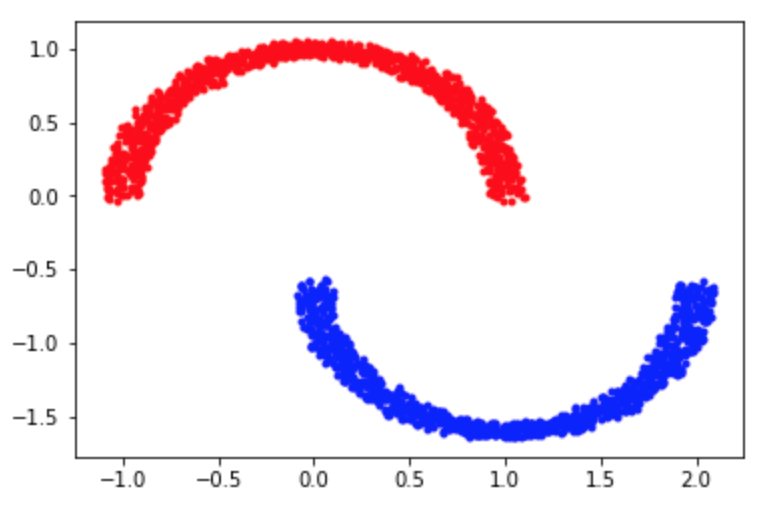
\includegraphics[width=0.6\textwidth]{3-1-a1.jpg}
    \end{center}
    \begin{center}
        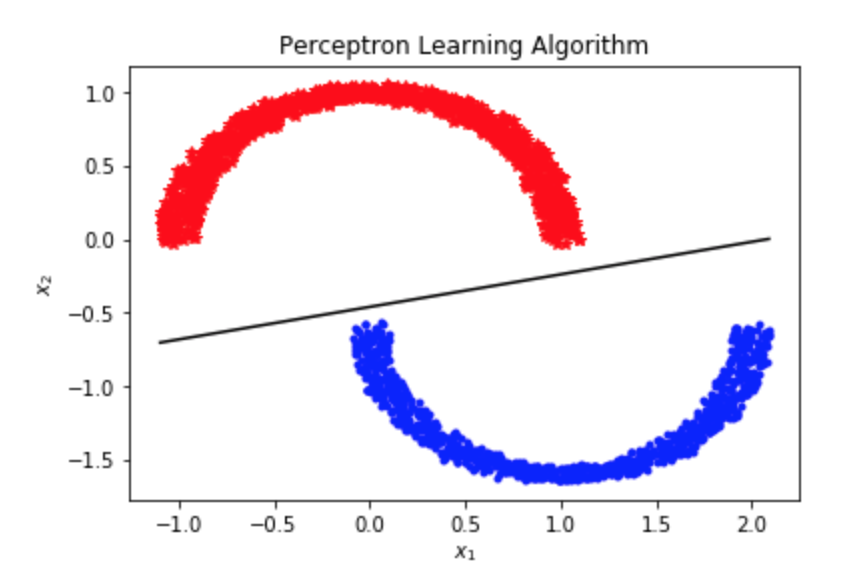
\includegraphics[width=0.6\textwidth]{3-1-a2.jpg}
    \end{center}
    \item[(b)] Repeat part (a) using the linear regression (for classification) to obtain 
    \textbf{w}.  Explain your observations.
    \begin{center}
        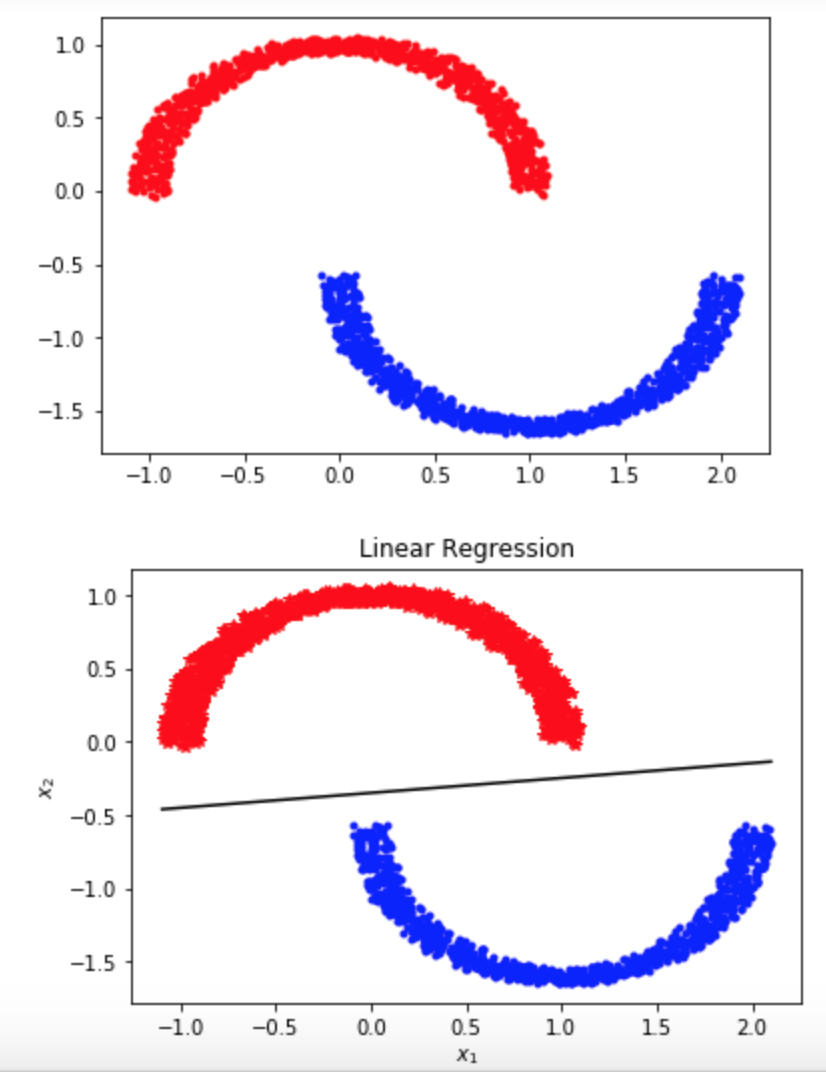
\includegraphics[width=0.6\textwidth]{3-1-b.jpg}
    \end{center}
    These are the results we obtain from repeating part (a) using the linear regression (for 
    classification) to obtain \textbf{w}.  As we can see there are a few slight differences 
    between the results but it shows us that we can use linear regression for this classification.  
    These new values of \textbf{w} still allow us to obtain an approximate solution for this model.

\end{itemize}

% ----------------------------------------------------------------------------------------------

\subsection{Problem 3.2 (extra credit)} For the double-semi-circle task in Problem 3.1, vary 
\textit{sep} in the range $\{0.2, 0.4, \ldots, 5\}$.  Generate $2,000$ examples and run the PLA 
starting with \textbf{w = 0}.  Record the number of iterations PLA takes to converge.\\
Plot \textit{sep} versus the number of iterations taken for PLA to converge.  Explain your 
observations.  [Hint: Problem 1.3]

\begin{center}
    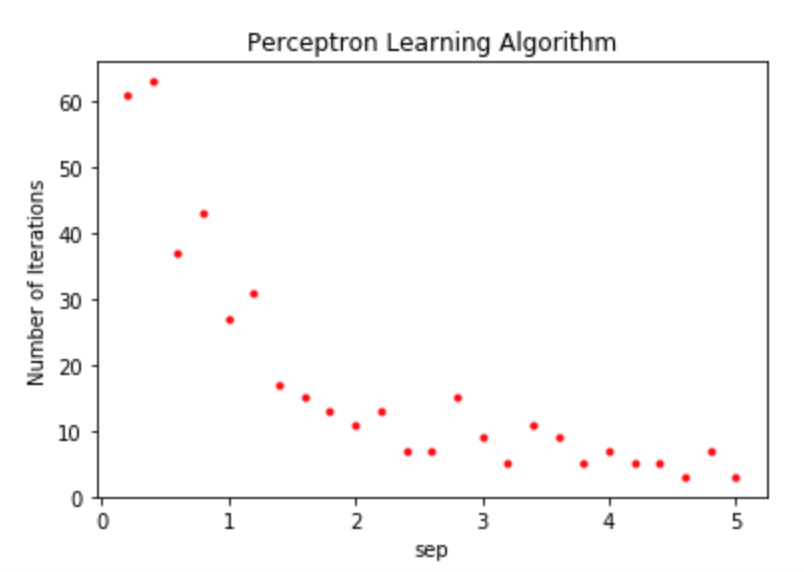
\includegraphics[width=0.6\textwidth]{3-2.jpg}
\end{center}
After plotting \textit{sep} versus the number of iterations taken for PLA to converge, we can see 
that it is decreasing as the \textit{sep} is increasing.  In other words, the more separated the 
semi-circles are, the faster the PLA can converge to a solution.

\end{document}
